\documentclass{exam}
\title{\textbf{Applied Regression Analysis}\large\\
	 \textbf{Homework 1}}

\author{Mitchell Matheny}
\usepackage{graphicx}
\graphicspath{ {images/} }
\usepackage{graphicx}
\graphicspath{ {images/} }
\usepackage{amsmath}
\usepackage{amssymb}







\begin{document}
	\maketitle{}
	For problems 6 through 10. I have typed out the short version of the work with solutions. The hand written work is attached at the end of this document. 
	\pagebreak
	\section{Exercise 1.1}
	The study used in this exercise looks at a study of teenage gambling in Britain. Make a numerical and graphical summary of the data, commenting on what you notice.
	\\
	When initially looking at the summary of the data. One notices that the number male and female entries are treated as numerical data. We therefor need to convert them into what is called a factor. This is accomplished by using the following command: 
	\\
	\\
	teengamb\$sex < - factor(teengamb\$sex)
	\\
	\\
	After doing so the summary looks like this: 
	
	\begin{figure}[h]
		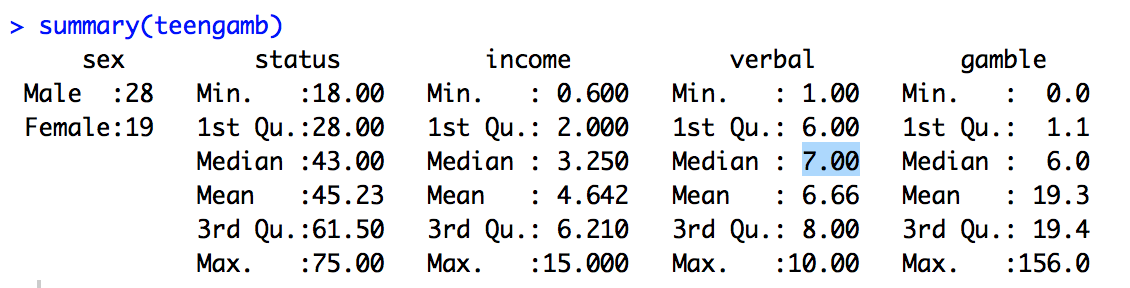
\includegraphics[scale=.6]{summary}
		\centering
		
	\end{figure}
	
	\noindent
	We can now easily see how many males and females where included in this study. This will also make it much easier to differentiate the sex on the various plots to follow. 
	\\
	\\
	\textbf{Comments on Numerical Summary and Univariate Plots}: 
	\\
	\\
	\textbf{Status}
	The numerical values for family status seem a bit arbitrary. The documentation doesn’t really specify how these numbers were calculated, this would take a bit more research into the actual study. With numerical values ranging from 18 to 75, both the mean and median are above the middle of the range of 40. Indicating that the societal status of the parents of the teenagers in this study are on the higher end of the spectrum. We can see this more clearly by looking at a histogram of the data:
	
	
	\begin{figure}[h]
		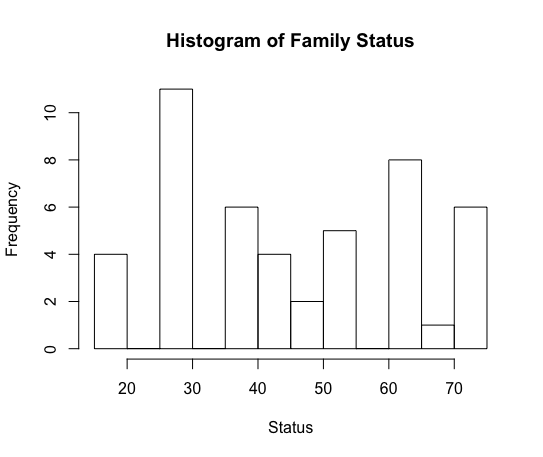
\includegraphics[scale=.5]{status}
		\centering
		
	\end{figure}
	As we can see, the majority of the participants have a status above 40. 
	\pagebreak
	
	\noindent
	\textbf{Income}:
	The numerical values for income are given in pounds per week. The average income is 4.6 pounds per week, which is equivalent to only \$6.16 U.S. This seems like a very low value compared to the average of 500 pounds per week (\$670 U.S), but considering that these are teenagers, the values seem acceptable. 
	Looking at the histogram: 
	
	\begin{figure}[h]
		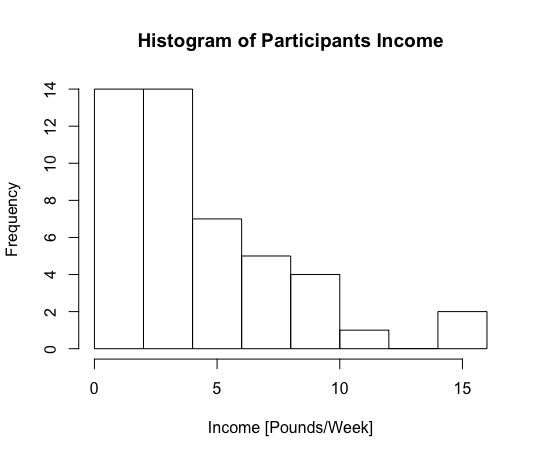
\includegraphics[scale=.5]{income}
		\centering
		
	\end{figure}
	
	\noindent
	We can see the the ~60\% of the participants make less than 5 pounds per week (\$6.69 U.S), and the average is screwed by the 2 participants making 15 pounds per week (\$20.00 U.S)
	\\
	\\
	\textbf{Verbal}:
	The verbal tests were scored on a scale of 0 to 12. Looking at the summary, we can see that the average value of 6.6 is just above the 50\% correct mark, possibly indicating that the scores are screwed towards the higher end of the scale. Looking at the histogram: 
	
	\begin{figure}[h]
		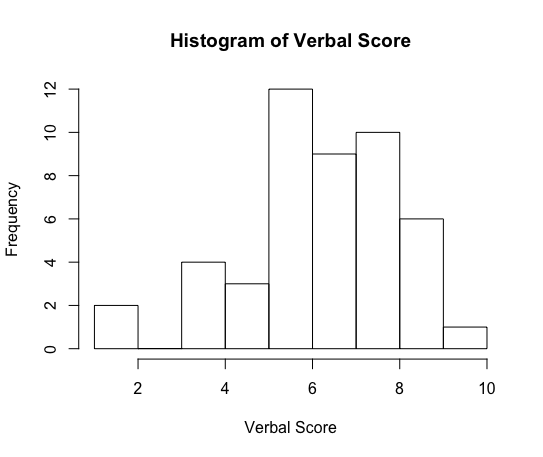
\includegraphics[scale=.5]{verbal}
		\centering
		
	\end{figure}
	
	\noindent
	We can clearly see that the majority of the participants scored 50\% or better. 
	\pagebreak
	
	\noindent
	\textbf{Gamble}:
	The participants reported the amount of money the spent on gambling in pounds per year. Looking at the summary, we can see that the values have a large range. The minimum being 0 pounds per year spent to 156 pounds spent per year. Due to the large maximum value the mean is shifted to a higher value of 19.3. We can see however that the majority of the participants spend little to no money on gambling as the median value is 6. Looking at the histogram, we can see that this is that case. 
	
	\begin{figure}[h]
		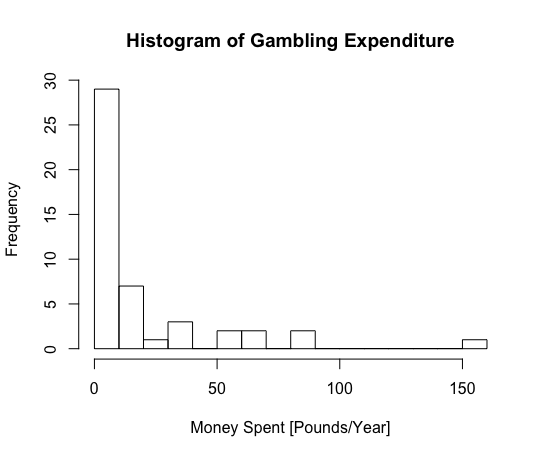
\includegraphics[scale=.5]{gamble}
		\centering
		
	\end{figure}
	
	\noindent
	\textbf{Multivariate Plots}
	
	\noindent
	For the Multivariate plots, I will only make comments on plots that i notice trends on.
	\\
	\\
	\\ 
	When looking at all of the plots relating a variable to sex, the only visually noticeable trend would be between the amount gambled per year: Men spent more per year than women. There is also a slight trend between the amount of money earned per week and the amount gambled per year. There appears to be a slight upward linear trend, indicating that the more earned per week, the more likely the participant was to spend money on gambling. This however is a speculation, and would need further analysis to confirm. 
	The last trend i noticed was there is a slight linear trend when comparing verbal scores and parental status. The participants with a higher family status tended to score higher on the verbal test. Further analysis is needed to determine the true relationship.  
 
\\
\\
\textbf{Plots are located after problems 6-10 } 





\begin{figure}[t!]
	\centering
	\begin{subfigure}
	\centering
	\includegraphics[scale = .7]{Gamble_v_sex}		
	\end{subfigure}%
	~ 
	\begin{subfigure}
	\centering
	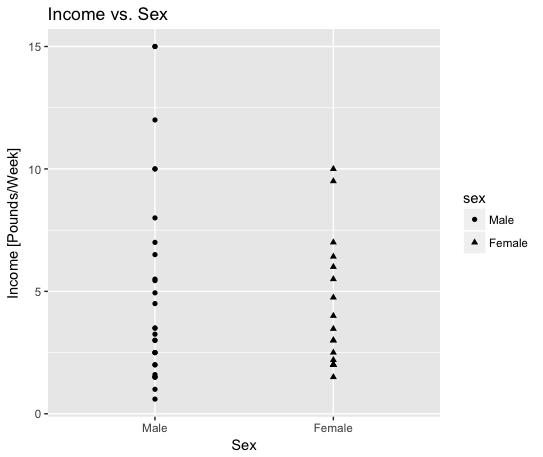
\includegraphics[scale=0.7]{Income_V_sex}
	\end{subfigure}
\end{figure}

\pagebreak
\begin{figure}[t!]
	\begin{subfigure}
	\centering
	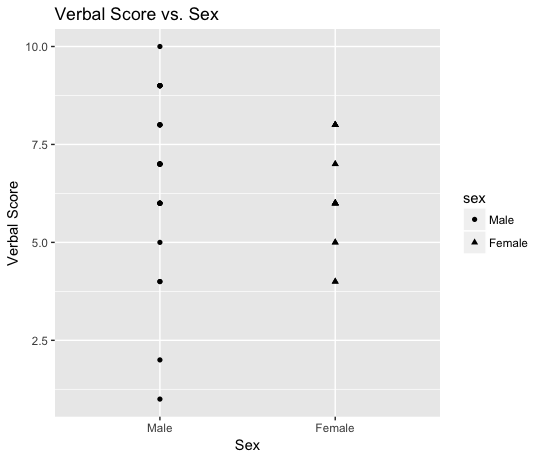
\includegraphics[scale=0.7]{Verbal_V_sex}
	\end{subfigure}
	~
	\begin{subfigure}
	\centering
	\includegraphics[scale=0.7]{Status_V_sex}
	\end{subfigure}

\end{figure}

\begin{figure}[t!]
	\centering
	\begin{subfigure}
		\centering
		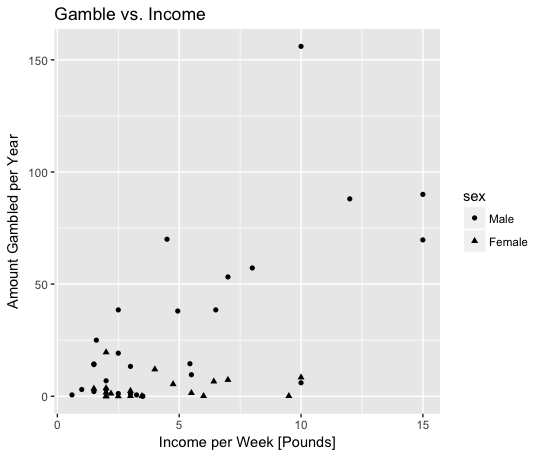
\includegraphics[scale = .7]{Gamble_V_income}		
	\end{subfigure}%
	~ 
	\begin{subfigure}
		\centering
		\includegraphics[scale=0.7]{Income_V_status}
	\end{subfigure}
\end{figure}

\pagebreak
\begin{figure}[t!]
	\begin{subfigure}
		\centering
		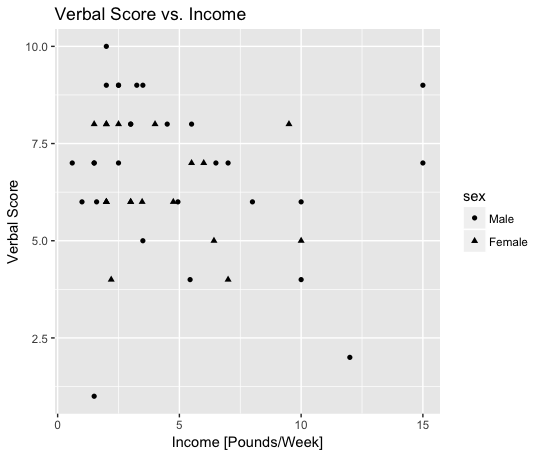
\includegraphics[scale=0.7]{Verbal_V_income}
	\end{subfigure}
	~
	\begin{subfigure}
		\centering
		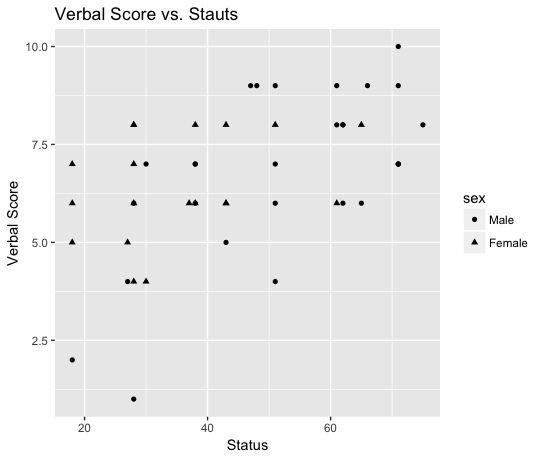
\includegraphics[scale=0.7]{Verbal_V_status}
	\end{subfigure}
	
\end{figure}

\pagebreak
\begin{figure}[t!]
	\begin{subfigure}
		\centering
		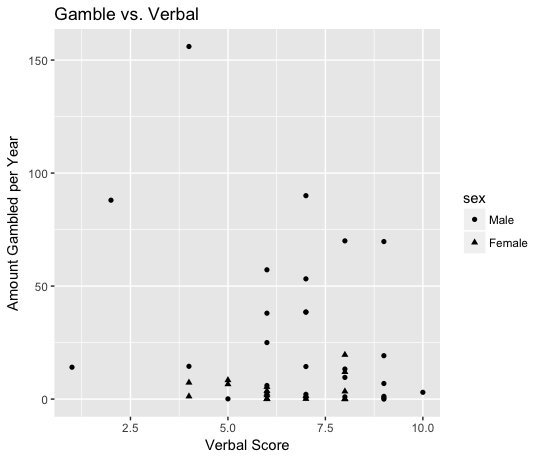
\includegraphics[scale=0.7]{Gamble_V_verbal}
	\end{subfigure}
	~
	\begin{subfigure}
		\centering
		\includegraphics[scale=0.7]{Gamble_V_Status}
	\end{subfigure}
	
\end{figure}

\pagebreak



\section{Problems 6-10}


\textbf{Problem 6}:
\\
\\
Suppose that Y is a random variable with pdf, $f(y) = \lambda e^{-\lambda y}$ Determing the mean and variance of Y.
\\
The mean is just the expectaion value.

\begin{equation}
\begin{gathered}
E[y] = \int y \lambda e^{-\lambda y}dy \\
\end{gathered}
\end{equation} 

\noindent
Solving via integration by parts, the mean is therefore:

\begin{equation}
\begin{gathered}
E[y] = \frac{-e^{-\lambda y}(\lambda y + 1)}{\lambda}
\end{gathered}
\end{equation} 
\\
\noindent
To find the Variance:

\begin{equation}
\begin{gathered}
Var[y] = E[y^2] - E[y]^2\\
\\
E[y^2] = \int y^2 \lambda e^{-\lambda y}dy = \frac{e^{-\lambda y}(\lambda^2 y^2 + 2\lambda y +2)}{\lambda^2}
\end{gathered}
\end{equation} 
\\
Therefore the variance:
\\
\begin{equation}
\begin{gathered}
Var[y] = \frac{e^{-\lambda y}(\lambda^2 y^2 + 2\lambda y +2)}{\lambda^2} + \frac{-e^{-2\lambda y}(\lambda y + 1)^2}{\lambda^2}
\end{gathered}
\end{equation} 
\\
\\
\noindent
\textbf{Problem 7}:
\\
\\
Determing the mean and variance of 4Y +2.
\\
\\
Using the following property: 
\begin{equation}
\begin{gathered}
E[aY + b] = aE[Y] +b\\
\\
E[4Y+2] = 4e[y] + 2\\
\end{gathered}
\end{equation} 
\\
Therefore the mean is: 
\begin{equation}
\begin{gathered}
E[4Y+2] = \frac{-4e^{-\lambda y}(\lambda y + 1)}{\lambda} +2
\end{gathered}
\end{equation} 
\\
\\
Using a similar argument for the variance: 

\begin{equation}
\begin{gathered}
Var[aY+b] = a^2Var[Y] = 16Var[Y]\\
\\
Var[4Y+2] =  \frac{16e^{-\lambda y}(\lambda^2 y^2 + 2\lambda y +2)}{\lambda^2} + \frac{-16e^{-2\lambda y}(\lambda y + 1)^2}{\lambda^2}
\end{gathered}
\end{equation}

\pagebreak


\textbf{Problem 8}: 
\\
\\
Suppose that random variables X and Y have a joint PDF given by $ f(x,y) = 6(1-y);0<=x<=y<=1.$ Determine $f_x,f_y,E(X),E(Y),E(XY), and cov(X,Y)$.

 \begin{equation}
 \begin{gathered}
f_x = \int_{x}^{1}(6-6y) dy\\
f_x = 3x^2 -6x +3\\
\\ 
f_y = \int_{0}^{y}(6-6y) dx\\
f_y = -6y^2 +6y\\
\\
E[x] = \int_{0}^{1}xf_x dx = \int_{0}^{1}(3x^3 - 6x^2 +3x) dx\\
E[x] = \frac{1}{4}\\
\\
E[y] = \int_{0}^{1}xf_y dy = \int_{0}^{1}y(-6y^2 +6y)dy\\
E[y] = \frac{1}{2}\\
\\
E[xy] = \int_{0}^{1} \int_{0}^{1} xyf(x,y)dxdy = \int_{0}^{1} \int_{0}^{1} xy(6-6y)dx dy\\
E[xy] = 1\\
\\
Cov[xy] = E[xy]-E[x]E[y]\\
Cov[xy] = \frac{7}{8}
 \end{gathered}
 \end{equation}

\pagebreak

\textbf{Problem 9}:
\\
\\
Suppose that $y = (Y_1,Y_2)^T$ is a bivariate normal random vectore with mean and variance;

\begin{equation}
\begin{gathered}
E[y] = \begin{pmatrix} 1 & 2 \end{pmatrix}^T\\
\\
Var[y] = \begin{pmatrix} 1 & 0.25 \\ 0.25 & 2 \end{pmatrix}
\end{gathered}
\end{equation}

What is the distribution, mean, and variance of $a^Ty$, where $a =\begin{pmatrix} 1 & 3 \end{pmatrix}^T $
\\
\begin{equation}
\begin{gathered}
f(y) =a^Ty = \begin{pmatrix} 1 & 3 \end{pmatrix} \begin{pmatrix} Y_1 \\ Y_2 \end{pmatrix}\\
f(y) = Y_1 + 3Y_2
\\
\end{gathered}
\end{equation}
\\
For the mean: 
\begin{equation}
\begin{gathered}
E[a^Ty] = a^TE[y]\\
E[a^Ty] = \begin{pmatrix} 1 & 3 \end{pmatrix} \begin{pmatrix} 1 \\ 2 \end{pmatrix}\\
\\
E[a^Ty] = 7
\\
\end{gathered}
\end{equation}
\\
For the variance: 

\begin{equation}
\begin{gathered}
Var[a^ty] = aVar[y]a^T\\
\\
Var[a^Ty] = 
\begin{pmatrix}1 & 3\end{pmatrix}
\begin{pmatrix} 1 & 0.25 \\ 0.25 & 2 \end{pmatrix} 
\begin{pmatrix} 1 \\ 3 \end{pmatrix}\\
\\
Var[a^ty] = 20.5
\end{gathered}
\end{equation}


\pagebreak
\textbf{Problem 10}:\\
\\
Using the same y as in problem 4, determone the distribution. mean, and variance of $z = Ay$, where 
\\
\begin{equation}
\begin{gathered}
A = \begin{pmatrix} 2 & 1 \\ 1 & 2 \end{pmatrix} 
\end{gathered}
\end{equation}
\\
\begin{equation}
\begin{gathered}
z = Ay =  \begin{pmatrix} 2 & 1 \\ 1 & 2 \end{pmatrix}\begin{pmatrix} Y_1\\Y_2 \end{pmatrix}\\
\\
z = \begin{pmatrix} 2Y_1+Y_2\\Y_1+2Y_2 \end{pmatrix}
\end{gathered}
\end{equation}
\\
For the mean: 
\begin{equation}
\begin{gathered}
E[AY] = AE[Y]\\
E[AY] = \begin{pmatrix} 2 & 1 \\ 1 & 2 \end{pmatrix}\begin{pmatrix} 1\\2 \end{pmatrix}\\
\\
E[AY] = \begin{pmatrix} 4\\3 \end{pmatrix}
\end{gathered}
\end{equation}
\\
For the Variance:
\begin{equation}
\begin{gathered}
Var[AY] = AVar[Y]A^T\\
\\
Var[AY] = \begin{pmatrix} 2 & 1 \\ 1 & 2 \end{pmatrix}\begin{pmatrix} 1 & 0.25 \\ 0.25 & 2 \end{pmatrix}\begin{pmatrix} 2 & -1 \\ -1 & 2 \end{pmatrix}\\
\\
Var[AY] = \begin{pmatrix} 3.5 & 2.5 \\ -0.5 & 6 \end{pmatrix}
\end{gathered}
\end{equation}







\end{document}




